% !TEX spellcheck = en_US

\documentclass[conference]{IEEEtran}
\usepackage{cite}
\usepackage{amsmath,amssymb,amsfonts}
\usepackage{algorithmic}
\usepackage{graphicx}
\usepackage{textcomp}
\usepackage{xcolor}
% add hyperlinks, delete all .aux files if adding hyperref after previous build
\usepackage{hyperref}
% support for unicode charcters like "é" and "ñ"
\usepackage[T1]{fontenc}
% Provides generic commands \degree, \celsius, \perthousand, \micro and \ohm
\usepackage{gensymb}
% splits a section into multiple columns
\usepackage{multicol}
\def\BibTeX{{\rm B\kern-.05em{\sc i\kern-.025em b}\kern-.08em
    T\kern-.1667em\lower.7ex\hbox{E}\kern-.125emX}}
\begin{document}

\title{Effects of Satellite Sampling on Subhourly Modeling errors}

\author{\IEEEauthorblockN{Mark A. Mikofski, Abhishek Parikh, and Jeffrey Newmiller}
\IEEEauthorblockA{DNV, Oakland, CA, 94612, USA }}

\maketitle

\begin{abstract}
Modeling errors due to hourly inputs averaged from high frequency measurements can be significant where solar resource variability and inverter loading ratios are both high. However, satellite data sources average low frequency measurements. This paper studies the effects of satellite sampling frequency on hourly modeling errors. Simulating satellite data from high frequency measurements by selecting instantaneous measurements at a lower sampling rate then averaging selected instantaneous measurements for the hour, we observe modeling errors with simulated satellite data sampled every 15-minutes or shorter, but for sampling rates at 30-minutes or longer, modeling errors appear to cancel out annually possibly due to random errors in the sampled data. Similar effects have been observed by other researchers, and the results of this study seem to confirm their findings. However, the modeling error is not completely canceled out. Even at sampling rates longer than 30-minutes, we still see some modeling error, and the modeling error increases as sampling rates get shorter. Based on our observations, we recommend that a modeling error correction be applied whenever hourly inputs are used, especially at sites with high solar variability and DC/AC ratios greater than one.
\end{abstract}

\begin{IEEEkeywords}
inverter, clipping, satellite, sampling, solar resource, irradiance, variability, performance, modeling, TMY
\end{IEEEkeywords}

\section{Introduction}
Accurate solar energy assessments are important for lowering the cost of capital for PV systems. However, continuing under-performance of solar assets over the past few years may be damaging investor confidence \cite{Matsui2021}. Several studies have examined potential sources of under-prediction, and subhourly modeling errors has recently received renewed interest \cite{Parikh2021,Anderson2020,Bradford2020,Kharait2020,Cormode2019}. Subhourly modeling errors arise from differences in predicted clipping losses and energy output between using hourly versus subhourly input. When hourly input is time-averaged from high-frequency subhourly measurements, energy output is over-predicted and clipping losses are under-predicted. However, satellite data is generated from low-frequency measurements that are sampled at 15-minute or 30-minute intervals \cite{Wilcox2012,Sengupta2018}. Recently, a few studies have investigated the difference between hourly input time-averaged from high-frequency versus input generated from low-frequency sampled data and have demonstrated that modeling errors appear to be reduced for slower sampled data \cite{Bowersox2021}. This study examines the impact of sampling rate on modeling error by simulating satellite data at various frequencies from high-frequency ground measurements at the NIST ground array \cite{Boyd2017,Boyd2017a,Boyd2017b}. The final paper will expand the study to also include simulated satellite data from the 7 SURFRAD stations \cite{Augustine2000}.

\section{Methods}
\subsection{Locations}
There are 7 SURFRAD stations \cite{Augustine2000} across \cite{Bowersox2021} the United States with 1 to 3 minute resolution. Fig.~ shows the SURFRAD site locations. We selected TMY2 \cite{Marion1995} and TMY3 \cite{Wilcox2012} sites within 120[km] from the SURFRAD site that did not have any significant monthly irradiance, temperature, or wind speed deviations from the other nearby datasets. The generic uncertainty for both TMY2 and TMY3 is 5-8\% at 95\% confidence. For each SURFRAD site the PSM3 was queried for the nearest location using pvlib python \cite{F.Holmgren2018}. Table~\ref{table:surfrad-tmy-location-summary} shows the station names, global coordinates, and metadata about each site. The error from the SURFRAD median in the last column will be discussed later in the results, Section~\ref{section:results}.

\begin{table*}[htbp]
\caption{Summary of SURFRAD, NSRDB, and TMY Locations}
\begin{center}
\begin{tabular}{|c|c|c|c|c|c|c|}
\hline
\textbf{Station}&\textbf{\textit{Latitude}}&\textbf{\textit{Longitude}}&\textbf{\textit{Elevation}}&\textbf{\textit{TMY}}&\textbf{\textit{ID}}&\textbf{\textit{Error}} \\
\hline
Bondville, IL&40.05&-88.37&213&SURFRAD&bon& \\
NSRDB&40.05&-88.38&213&PSM3&887015&8.9\% \\
SPRINGFIELD, IL&39.83333333&-89.66666667&187&TMY2&93822&4.9\% \\
SPRINGFIELD CAPITAL AP&39.85&-89.683&179&TMY3&724390&2.9\% \\
\hline
Boulder, CO&40.13&-105.24&1689&SURFRAD&tbl& \\
NSRDB&40.13&-105.22&1616&PSM3&150658&1.3\% \\
BOULDER, CO&40.01666667&-105.25&1634&TMY2&94018&1.9\% \\
DENVER INTL AP&39.833&-104.65&1650&TMY3&725650&0.6\% \\
AURORA BUCKLEY FIELD ANGB&39.717&-104.75&1726&TMY3&724695&0.8\% \\
DENVER/CENTENNIAL [GOLDEN - NREL]&39.742&-105.179&1829&TMY3&724666&-1.8\% \\
\hline
Desert Rock, NV&36.62&-116.02&1007&SURFRAD&dra& \\
NSRDB&36.61&-116.02&991&PSM3&109824&4.0\% \\
MERCURY DESERT ROCK AP [SURFRAD]&36.63&-116.02&935&TMY3&723870&1.0\% \\
\hline
Fort Peck, MT&48.31&-105.1&634&SURFRAD&fpk& \\
NSRDB&48.33&-105.1&629&PSM3&250489&3.0\% \\
GLASGOW, MT&48.21666667&-106.6166667&700&TMY2&94008&1.6\% \\
GLASGOW INTL ARPT&48.217&-106.617&699&TMY3&727680&2.3\% \\
\hline
Goodwin Creek, MS&34.25&-89.87&98&SURFRAD&gwn& \\
NSRDB&34.25&-89.86&95&PSM3&852772&13.3\% \\
MEMPHIS, TN&35.05&-89.98333333&87&TMY2&13893&6.5\% \\
GREENWOOD LEFLORE ARPT&33.5&-90.083&47&TMY3&722359&3.9\% \\
GREENVILLE MUNICIPAL&33.483&-90.983&42&TMY3&722356&3.4\% \\
MEMPHIS INTERNATIONAL AP&35.067&-89.983&81&TMY3&723340&2.9\% \\
COLUMBUS AFB&33.65&-88.45&68&TMY3&723306&-1.6\% \\
\hline
Penn State, PA&40.72&-77.93&376&SURFRAD&psu& \\
NSRDB&40.73&-77.94&378&PSM3&1116869&8.8\% \\
WILLIAMSPORT, PA&41.26666667&-77.05&243&TMY2&14778&-2.5\% \\
DUBOIS FAA AP&41.183&-78.9&553&TMY3&725125&-5.5\% \\
\hline
Sioux Falls, SD&43.73&-96.62&473&SURFRAD&sxf& \\
NSRDB&43.73&-96.62&479&PSM3&706377&6.1\% \\
SIOUX FALLS, SD&43.56666667&-96.73333333&435&TMY2&14944&1.8\% \\
SIOUX FALLS FOSS FIELD&43.583&-96.75&433&TMY3&726510&0.4\% \\
BROOKINGS (AWOS)&44.3&-96.817&502&TMY3&726515&-3.5\% \\
\hline
\end{tabular}
\label{table:surfrad-tmy-location-summary}
\end{center}
\end{table*}

\subsection{Annual Energy Prediction}
We used pvlib python \cite{F.Holmgren2018} to calculate the solar position for each site and the rotations for a fictitious single-axis tracker system. We used the SURFRAD measured global horizontal irradiance (GHI) and decomposed it into direct normal irradiance (DNI) and diffuse horizontal irradiance \cite{ERBS1982293}, then transposed it to the plane of the array (POA) accounting for diffuse components, ground reflection, and incidence angle modifiers \cite{HayDavies}. We assume isotropic sky diffuse and an albedo of 0.25 for ground diffuse. To get the effective irradiance, we combined the POA components applying the ASHRAE incidence angle modifiers with $b_0=0.05$ to the direct irradiance and neglected spectral mismatch. Because SURFRAD doesn't include ambient temperature, we used RdTools \cite{Jordan2018} to get clear sky temperatures, and then scaled it to the daily ratio of SURFRAD GHI to calculated clear sky GHI \cite{Ineichen2002} using (\ref{eq:adjusted-temperature}). We used the PVsyst model to estimate module cell temperatures with default coefficients, $U_c=29, U_v=0$, the adjusted air temperature, and zero wind speed \cite{Faimain2008}. Finally, we predicted the DC power for a representative 300[W] mono-crystalline silicon module (Canadian Solar CS6X-300M) with the CEC 6-parameter model \cite{Dobos2012}. Then we resampled the data at hourly frequency and summed each day (\ref{eq:daily-energy}) and year (\ref{eq:annual-energy}). All years that had less than 350 days were removed and the annual energy was scaled to a full year accounting for leap years. We normalized by the module nameplate of 300[W] to get daily and annual DC capacity factors (CP) using (\ref{eq:daily-capacity-factor}) and (\ref{eq:annual-capacity-factor}). Then we repeated the simulations with PSM3 \cite{Habte2017}, TMY2 \cite{Marion1995}, and TMY3 \cite{Wilcox2012}, but using the measured ambient temperature provided in the data set. The full model is available online (https://github.com/mikofski/PVRW2021).

\begin{equation}
\begin{aligned}
T_{adj} &= T_{clearsky} + \left(\frac{GHI}{GHI_{clearsky}} - 1 \right)\Delta T \\
\Delta T &= T_{max,daily} - T_{min,daily} 
\end{aligned}
\label{eq:adjusted-temperature}
\end{equation}

\begin{equation}
E_\text{daily} = \sum_\text{time=1AM}^\text{12AM}{E_\text{hourly}} \label{eq:daily-energy}
\end{equation}

\begin{equation}
\mathit{CP}_\text{daily} = \frac{E_\text{daily}}{ 24\text{[h]} \text{Nameplate[W]} } \label{eq:daily-capacity-factor}
\end{equation}

\begin{equation}
E_\text{annual }= \sum_\text{day=1}^\text{365}{E_\text{daily}} \label{eq:annual-energy}
\end{equation}

\begin{equation}
\mathit{CP}_\text{annual} = \frac{E_\text{annual}}{ 8760\text{[h]} \text{Nameplate[W]} } \label{eq:annual-capacity-factor}
\end{equation}

\section{Results}
\label{section:results}

\subsection{Analysis}
We plotted histograms of the annual predictions using SURFRAD data for each of the 7 sites in. The top plot shows the daily capacity factors (\ref{eq:daily-capacity-factor}) and annual capacity factors overlaid in red (\ref{eq:annual-capacity-factor}), while the bottom plot shows the histogram of annual energy per module (\ref{eq:annual-energy}) with the median (P50) and 90\% chance of exceedance (P90) marked with dashed blue lines. Then we overlaid the predicted PSM3, TMY2, and TMY3 predictions and annotated the plot with their quantiles.

\begin{figure}[htbp]
\centerline{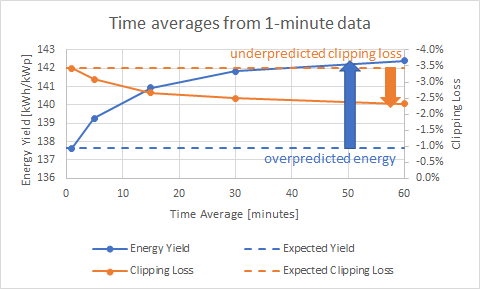
\includegraphics[width=9cm]{time-averaged.png}}
\caption{Daily (blue) and annual (red) capacity factor relative to DC nameplate for Bondville, IL, SURFRAD site (top) and distribution of annual DC energy per module (bottom).}
\label{fig:time-averaged}
\end{figure}

\begin{figure}[htbp]
\centerline{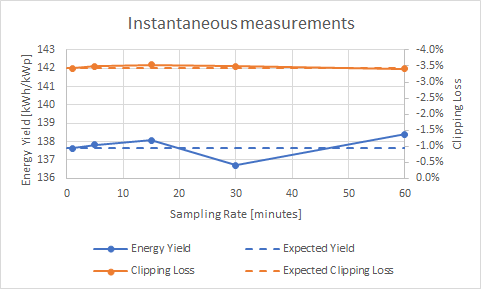
\includegraphics[width=9cm]{instantaneous.png}}
\caption{Daily (blue) and annual (red) capacity factor relative to DC nameplate for Boulder, CO, SURFRAD site (top) and distribution of annual DC energy per module (bottom).}
\label{fig:instantaneous}
\end{figure}

\begin{figure}[htbp]
\centerline{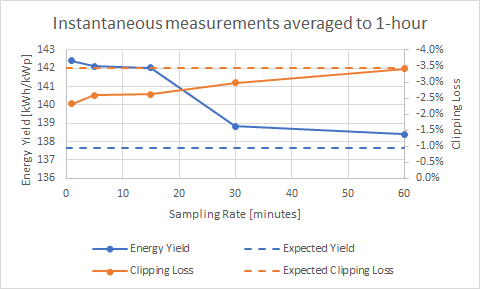
\includegraphics[width=9cm]{satellite-simulated.png}}
\caption{Daily (blue) and annual (red) capacity factor relative to DC nameplate for Desert Rock, NV, SURFRAD site (top) and distribution of annual DC energy per module (bottom).}
\label{fig:satellite-simulated}
\end{figure}

Table~\ref{table:surfrad-tmy-errors-summary} shows the relative differences between the TMY annual prediction and the SURFRAD median (\ref{eq:tmy-surfrad-median-error}) so that positive errors mean the TMY overpredicted. Table~\ref{table:surfrad-tmy-summary} summarizes the results as annual capacity factors (\ref{eq:annual-capacity-factor}), and Table~\ref{table:surfrad-tmy-quantile-summary} summarizes the results as quantiles. Where more than one TMY3 was close to the SURFRAD station, the closest to the median is shown in the tables. The relative differences for all sites are shown in the last column of Table~\ref{table:surfrad-tmy-location-summary}.

\begin{equation}
Error = \frac{CP_{TMY}}{CP_{SURFRAD,P50}}-1 \label{eq:tmy-surfrad-median-error}
\end{equation}

\begin{table}[htbp]
\caption{Summary of Differences Between SURFRAD median and TMY Annual Predictions}
\begin{center}
\begin{tabular}{|c|c|c|c|}
\hline
\textbf{Station}&\textbf{\textit{PSM3}}&\textbf{\textit{TMY2}}&\textbf{\textit{TMY3}} \\
\hline
bon&8.9\%&4.9\%&2.9\% \\
tbl&1.3\%&1.9\%&0.6\% \\
dra&4.0\%&     &1.0\% \\
fpk&3.0\%&1.6\%&2.3\% \\
gwn&13.3\%&6.5\%&-1.6\% \\
psu&8.8\%&-2.5\%&-5.5\% \\
sxf&6.1\%&1.8\%&0.4\% \\
\hline
AVG&6.5\%&2.4\%&0.0\% \\
STD&4.2\%&3.1\%&2.8\% \\
\hline
\end{tabular}
\label{table:surfrad-tmy-errors-summary}
\end{center}
\end{table}

\begin{table}[htbp]
\caption{Summary of Predicted SURFRAD Annual Capacity Factors Compared with TMY}
\begin{center}
\begin{tabular}{|c|c|c|c|c|c|}
\hline
\textbf{SURFRAD Station} & \textbf{\textit{P50}}& \textbf{\textit{P90}}& \textbf{\textit{PSM3}}& \textbf{\textit{TMY2}}& \textbf{\textit{TMY3}} \\
\hline
Bondville, IL    & 20.2\%& 18.7\%& 21.9\%& 21.1\%& 20.7\% \\
Boulder, CO      & 23.4\%& 22.9\%& 23.7\%& 23.8\%& 23.5\% \\
Desert Rock,NV   & 28.6\%& 27.5\%& 29.7\%&       & 28.8\% \\
Fort Peck, MT    & 20.3\%& 19.5\%& 21.0\%& 20.7\%& 20.8\% \\
Goodwin Creek, MS& 21.1\%& 19.7\%& 23.9\%& 22.5\%& 20.8\% \\
Penn State, PA   & 18.6\%& 17.2\%& 20.2\%& 18.1\%& 17.5\% \\
Sioux Falls, SD  & 20.7\%& 19.6\%& 22.0\%& 21.1\%& 20.8\% \\
\hline
\end{tabular}
\label{table:surfrad-tmy-summary}
\end{center}
\end{table}

\begin{table}[htbp]
\caption{Summary of TMY Quantiles of SURFRAD Years}
\begin{center}
\begin{tabular}{|c|c|c|c|c|c|}
\hline
\textbf{SURFRAD Station} & \textbf{\textit{PSM3}}& \textbf{\textit{WBAN}}& \textbf{\textit{TMY2}}& \textbf{\textit{USAF}}& \textbf{\textit{TMY3}} \\
\hline
Bondville, IL    & 96.2\%& 93822&  88.5\%&724390&  88.5\% \\
Boulder, CO      & 56.0\%& 94018&  64.0\%&725650&  52.0\% \\
Desert Rock, NV  & 100\% &      &        &723870&  81.8\% \\
Fort Peck, MT    & 88.0\%& 94008&  76.0\%&727680&  80.0\% \\
Goodwin Creek, MS& 100\% & 13893&  92.3\%&723306&  46.2\% \\
Penn State, PA   & 100\% & 14778&  36.4\%&725125&  13.6\% \\
Sioux Falls, SD  & 94.1\%& 14944&  70.6\%&726510&  58.8\% \\
\hline
\end{tabular}
\label{table:surfrad-tmy-quantile-summary}
\end{center}
\end{table}

\subsection{Discussion}
It's difficult to spot any trends in the 20 or more years of data at each of the SURFRAD sites, compared to trends seen in other studies \cite{Muller2014}. Although there are some biases detected between the SURFRAD data and the oldest data set, TMY2 1960-1990 \cite{Marion1995}, the average difference from Table~\ref{table:surfrad-tmy-errors-summary}, 2.4\%, is on the same order as the standard deviation between the sites, 3.1\%, and is therefore inconclusive. The newer data set, TMY3 1990-2010 \cite{Wilcox2012}, seems closer to the SURFRAD data, 0\% average difference, but the standard deviation between sites, 2.8\%, is similar to the spread for the TMY2, so they appear to overlap and are not clearly distinguishable. The newest data surprisingly is an outlier with an average difference twice as big as for TMY2, 6.5\%, and a spread on the same order as TMY2 and TMY3, 4.2\%, so there's a clear distinction between it and the other datasets. More investigation is necessary to understand the difference.

The distribution of years differs between SURFRAD sites, perhaps due to climate differences. Bondville, IL, Fig.~\ref{fig:time-averaged} and Sioux Falls, SD, Fig.~\ref{fig:instantaneous} seem to be the most normal and symmetrical with ranges of about 10\%, but not all of the histograms show a normal distribution, some are flatter, many skewed, and some possibly multimodal. The range varies from site to site, between 5-10\%. Fort Peck, MT, has the closest range between 510-560[kWh/yr] per module. Desert Rock, NV, Fig.~\ref{fig:satellite-simulated} also has a tight range and the highest output of all the sites, but also has a long downside tail. The year 2002 is an outlier at this site and is about 50[kWh/yr] per module lower than the other years. Goodwin Creek, MS, also has a long downside tail and apparently no upside or a double peak. The years 2004 and 2014 are outliers in this data set deviating by nearly 20-25\% from previous and later years.

These SURFRAD sites do not cover all of the climates and regions in the US consistently. Most of the sites are in the interior, and there is a high concentration in the midwest. The average annual DC capacity factor is about 20\% with Desert Rock, NV, the exception at 28\%. There are no SURFRAD sites in the northwest, along the Pacific Coast, along the Gulf of Mexico, the Atlantic coast, or in the southeast, and there is only one site in the southwest, where there may be a high concentration of PV systems. For example Arizona or New Mexico. Therefore, the results of this study are limited and should not be extrapolated or applied uniformly to the entire United States.

\section{Conclusions}
We studied the question of whether TMY datasets are representative of the median predicted PV performance by comparing PV system simulations using TMY data with simulations using over 20 years of high-frequency, accurate, ground based SURFRAD measurements at 7 sites across the United States. We found that the TMY datasets all overpredicted the median SURFRAD annual performance at 5 of 7 sites. The PSM3 predictions were greater than the median for all sites, and greater than 90\% of years in 5 of 7 sites. TMY2 predictions were greater than 30-90\% of years at 6 sites except Desert Rock, NV which had no nearby TMY2 station. On average TMY3 predictions were closest to the SURFRAD median. Differences between the SURFRAD median and both TMY2 and TMY3 were within their uncertainties. Due to the lack of number of SURFRAD stations it is difficult to conclude whether there is a \textit{generic} high bias for TMY data. Although there is trend of generic high bias for PSM3 data, it is important to consider all available datasets and scrutinize them to determine the viability of long-term representative datasets. The distribution of differences from the SURFRAD median for both TMY2 and TMY3 stations were indiscernible; hence careful analysis is required to determine their utility in determining a long-term data set.

\bibliographystyle{IEEEtran}
% argument is your BibTeX string definitions and bibliography database(s)
\bibliography{IEEEabrv,bibliography}

\end{document}
